\chapter{Un dígito hecho de Sol -- II}

\lettrine[lines=2]{C}{ecilia volvió a} considerar los dígitos hechos
de pixeles abiertos y cerrados en una disposición matricial. Sabía que
de alguna manera debía decidir si cada pixel tenía que estar abierto o
cerrado. Pero no acertaba a saber cómo.

\begin{figure}[ht]
  \centering
  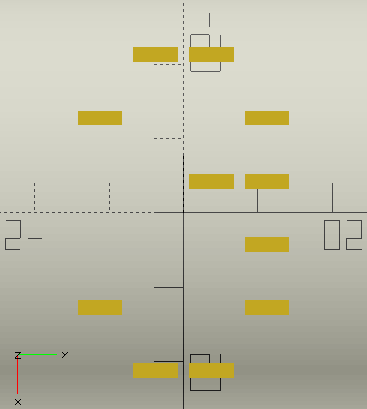
\includegraphics[height=.3\textwidth]{imagenes/tres}
  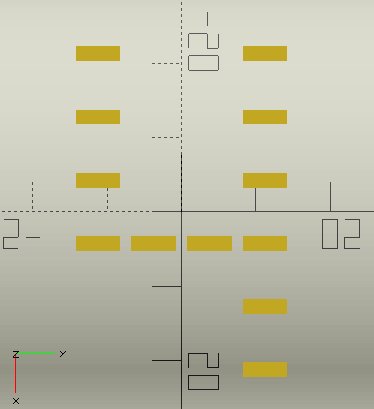
\includegraphics[height=.3\textwidth]{imagenes/cuatro}
  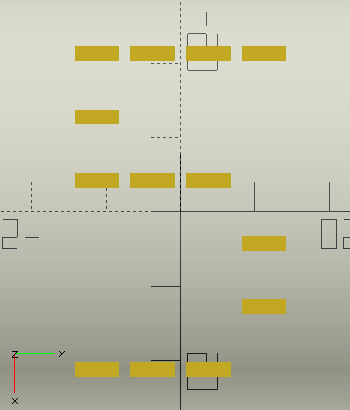
\includegraphics[height=.3\textwidth]{imagenes/cinco}
  \caption{Algunos digitos solares.}
\end{figure}


---El asunto no es sencillo ---concedió Antonia---;
pero por eso mismo es más interesante.

Tras una pausa, en la que pareció buscar la mejor manera de ayudar a
Cecilia sin caer en un \emph{espoiler}, continuó:

---Deberíamos ser capaces de recorrer cada fila y columna de la matriz
completa, pero en cada paso decidir (mediante un \lstinline!if!) si el
pixel en cuestión debe ser creado o no. Te recuerdo el módulo que
creaba toda la matriz; lo escribimos en el capítulo
\ref{sec:digito-solar-i}:

%    \begin{center}
 % \begin{minipage}[]{1\textwidth}%\vspace{0pt}
    \begin{lstlisting}
alto_pixel  = 2;
ancho_pixel = 6;      
delta_alto  = 6.5;
delta_ancho = 1.5;

module digito(alfa){
  for(i=[0:5],j=[0:3]){
   x=(i-2.5)*(alto_pixel+delta_alto);
   y=(j-1.5)*(ancho_pixel+delta_ancho);
   translate([x,y,-0.01])
    rayo_de_sol(alfa);
  } 
}

digito(alfa=90);
\end{lstlisting}

\begin{figure}[ht]
  \centering
  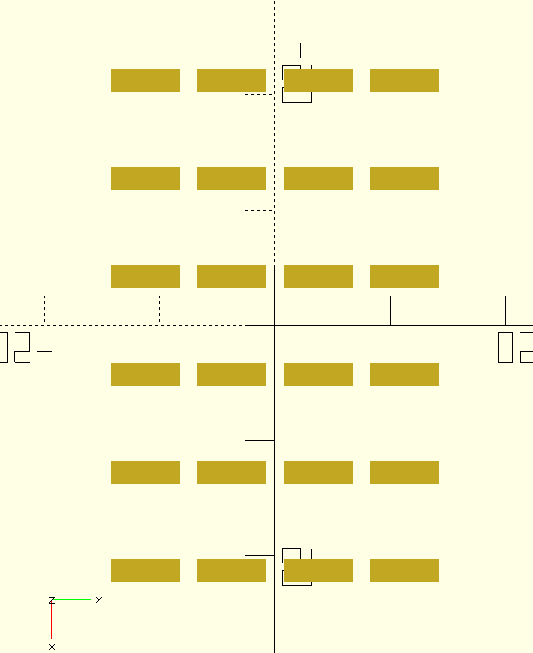
\includegraphics[width=.36\textwidth]{imagenes/matriz-completa-centrada-0}
  \caption{Matriz completa de rayos de Sol.}
  \label{fig:matriz-completa-centrada-1}
\end{figure}


Cecilia contempló ensimismada su texto. Recordó que cada pixel tenía
como nombre secreto sus coordenadas, tal como podía apreciar en la
figura \ref{fig:matriz-posiciones-y-dos-a}. Para el caso del dígito
`2', por ejemplo, los pixeles que debían crearse eran los mostrados en
la figura \ref{fig:matriz-posiciones-y-dos-b}.    

\begin{figure}[ht]
  \centering
  \subbottom[Matriz completa.\label{fig:matriz-posiciones-y-dos-a}]
  {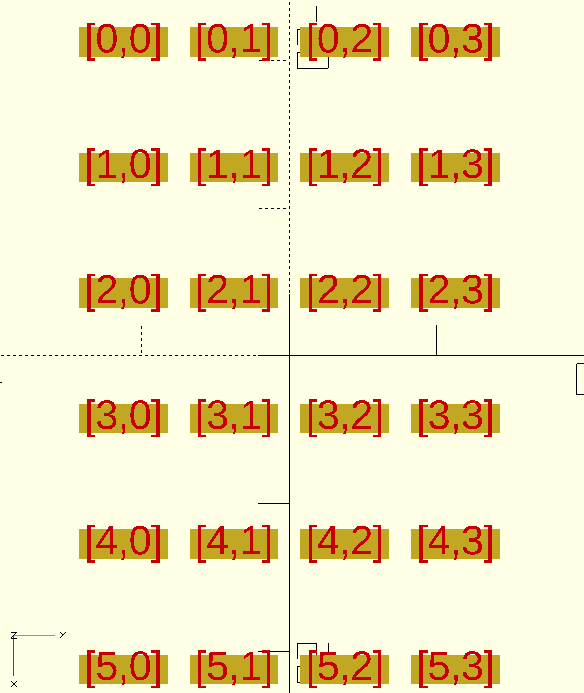
\includegraphics[width=.35\textwidth]{imagenes/matriz-posiciones}}
  \hspace{.1\textwidth}
  \subbottom[Dígito \texttt{2}.\label{fig:matriz-posiciones-y-dos-b}]
  {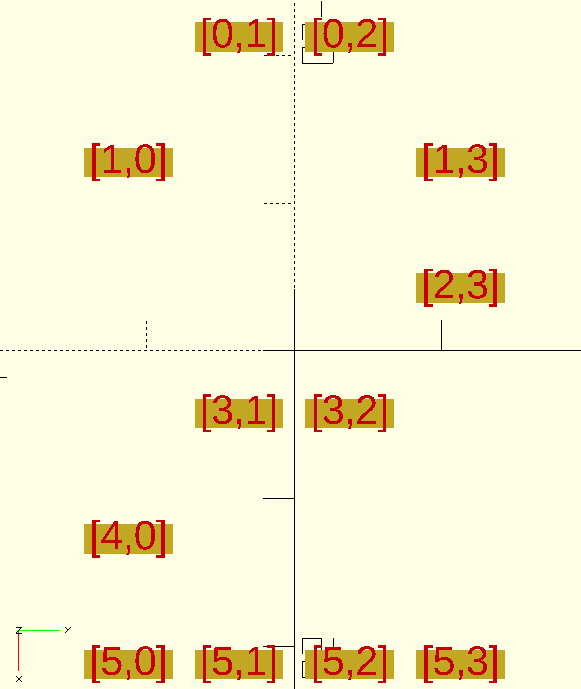
\includegraphics[width=.35\textwidth]{imagenes/dos-coordenadas}}
  \caption{Coordenadas de los rayos de Sol que forman un dígito.}
  \label{fig:matriz-posiciones-y-dos}
\end{figure}



\section{La manera de Cecilia}

Cecilia cruzó los brazos sobre su pecho, frunciendo el ceño y
recostándose con cierta frustración contra el respaldo de su silla: no
veía cómo plasmar esa idea en palabras. Pero de pronto una luz, sin
que supiera bien de dónde, cruzó su mente como un relámpago: <<¿Y si
paso esas coordenadas como un vector al módulo, y en lugar de pedirle
que recorra toda la matriz, le exijo que sólo cree los pixeles cuyas
coordenadas forman parte del vector...?>>. Presa de un súbito
entusiasmo, se lanzó sobre el teclado. Luego de unos cuantos minutos,
cuya cantidad no hubiera podido precisar, y que incluyeron varias
apelaciones a las siempre fieles teclas \keystroke{Supr} y
\keystroke{$\Longleftarrow$}, obtuvo lo siguiente:

     \begin{lstlisting}
dos=[[0,1], [0,2], [1,0], [1,3], [2,3], [3,1], [3,2], [4,0], [5,0], [5,1], [5,2], [5,3]];

module digito(alfa,numero){
  for(coords=numero){
    x=(coords[0]-2.5)*(alto_pixel+delta_alto);
    y=(coords[1]-1.5)*(ancho_pixel+delta_ancho);
    translate([x,y,-0.01])
      rayo_de_sol(alfa);
  }
}

digito(90,dos);
\end{lstlisting}

\begin{figure}[ht]
  \centering
  \includegraphics[width=.4\textwidth]{imagenes/dos-cecilia}  
  \caption{Dígito \texttt{2} logrado por Cecilia.}
  \label{fig:dos-cecilia}
\end{figure}

Cecilia estuvo a punto de gritar de alegría. Lentamente repasó su
texto, con los ojos radiantes de emoción: En la línea 1 definía un
vector, cuyos elementos eran las coordenadas de cada uno de los
pixeles que formaban el dígito ``2''.

El módulo recibía como parámetro ese vector con el nombre
\lstinline!numero!, y en la línea 4 lo recorría asignando cada par de
sus coordenadas a la variable \lstinline!coords!; de esta manera,
\lstinline!coords! valía primero \lstinline![0,1]!, después
\lstinline![0,2]!, luego \lstinline![1,0]!, etc.

Para cada valor de \lstinline!coords! se calculaban en las líneas 5 y
6 un par de \lstinline!x! e \lstinline!y!, usando para eso las dos
componentes de cada \lstinline!coords!: \lstinline!coords[0]! y
\lstinline!coords[1]!. Lo demás, se desprendía de la lógica de su
versión anterior del mismo módulo.

Cecilia giró sobre sí misma para mirar a Antonia:

---¿Ves?  Ahora sólo resta que escribamos los vectores para cada
dígito... ¡Y listo!  Ya podremos entonces escribir
\lstinline!digito(angulo,cero)!, \lstinline!digito(angulo,uno)!,
\lstinline!digito(angulo,dos)!, etc.

Antonia no demostraba la emoción que Cecilia esperaba; de hecho, no
mostraba ningún tipo de emoción: sólo miraba atentamente el monitor,
con gesto serio y concentrado. Cecilia pensó que en su texto había un
\emph{bug} oscuro y secreto, y que Antonia buscaba la manera de
revelárselo sin herir su sensibilidad.

Antonia pareció emerger lentamente de sus pensamientos. Volviendo la
mirada en dirección a Cecilia, pronunció suavemente:

---Muy bien. Está muy bien resuelto, de hecho. No es la forma en que
lo había hecho yo. Te confieso que me sorprende que hubiera otra
manera.

Cecilia sintió que la atravesaba una especie de escalofrío: ¿Había
encontrado otra forma? Inmediatamente reconoció la naturaleza de la
sensación que recorría su cuerpo: era el delicioso vértigo de la
independencia; el descubrimiento de que una era capaz de avanzar sin
la necesidad de ayuda. No era la primera vez que le ocurría: sintió lo
mismo cuando advirtió que su trabajo sobre los espectros estelares
cobraba finalmente forma, y supuso que la misma sensación la embargó
cuando se largó a dar sus primeros pasos, abandonando los brazos de su
madre.

---¿Me contás cómo lo hiciste vos? ---preguntó Cecilia con la misma
suavidad.

     
---Por supuesto ---respondió con una sonrisa Antonia, que ahora
parecía mirarla con otros ojos---. Primero dejame aprovechar para
comentarte acerca de una manera alternativa de referirse a los
elementos de un vector. Dado que muchas veces se usan para indicar
coordenadas --tal fue tu caso, de hecho--, los creadores de
\openscad{} decidieron incluir la posibilidad de que los tres primeros
elementos de un vector puedan llamarse usando la notación
`\lstinline!vector.x!', `\lstinline!vector.y!' y
`\lstinline!vector.z!':
     


\begin{lstlisting}
dos=[[0,1], [0,2], [1,0], [1,3], [2,3], [3,1], [3,2], [4,0], [5,0], [5,1], [5,2], [5,3]];

module digito(alfa,numero){
  for(coords=numero){
    x=(coords.x-2.5)*(alto_pixel+delta_alto);
    y=(coords.y-1.5)*(ancho_pixel+delta_ancho);
    translate([x,y,-0.01])
      rayo_de_sol(alfa);
  }
}
digito(90,dos);
\end{lstlisting}

% \begin{figure}[ht]
%   \centering
%   \includegraphics[width=.3\textwidth]{imagenes/dos-cecilia}  
% %  \caption{Dígito ``2'' logrado por Antonia.}
%   \label{fig:dos-antonia}
% \end{figure}

\guillemotright O sea, \lstinline!coords[0]! equivale a
\lstinline!coords.x! y \lstinline!coords[1]! a \lstinline!coords.y!;
no es más que un poco de `azúcar sintáctico', como suele decirse en el
ámbito de este género literario que es la programación... pero a veces
resulta expresivo ---reconoció Antonia, encogiéndose de hombros.

---Me gusta ---dijo Cecilia, que estaba de muy buen humor.

\section{La manera de Antonia}


---Te cuento cómo lo pensé yo ---comenzó Antonia---.  En mi mente,
visualizaba los dígitos como pixeles apagados y encendidos. Entonces
se me ocurrió replicar esa imagen mental con una suerte de `copia'
matricial, donde cada pixel encendido estuviera representado por un
`1' y los demás con un `0':

\begin{lstlisting}
dos=[[0, 1, 1, 0],
     [1, 0, 0, 1],
     [0, 0, 0, 1],
     [0, 1, 1, 0],
     [1, 0, 0, 0],
     [1, 1, 1, 1]];
\end{lstlisting}

\guillemotright La elección de los números 0 y 1 es caprichosa;
supongo que como programadora me siento más inclinada por todo lo que
parezca binario ---reconoció Antonia, y continuó---: Ahora bien, al
momento de recorrer filas y columnas, me fijaba si el correspondiente
elemento de la matriz era igual a `1': en caso afirmativo, creaba el
pixel; si no, no:


\begin{lstlisting}
module digito(alfa,numero){
  for(i=[0:5],j=[0:3]){
    if(numero[i][j]==1){
      x=(i-2.5)*(alto_pixel+delta_alto);
      y=(j-1.5)*(ancho_pixel+delta_ancho);
      translate([x,y,-0.01])
        rayo_de_sol(alfa);
    }
  }
}
digito(90,dos);
\end{lstlisting}

\begin{figure}[ht]
  \centering
  \includegraphics[width=.39\textwidth]{imagenes/dos-cecilia}  
  \caption[Dígito \texttt{2} conseguido por Antonia.]{Dígito
    `\texttt{2}' conseguido por Antonia. Como puede comprobarse, el
    resultado coincide con el conquistado por Cecilia.}
  \label{fig:dos-antonia}
\end{figure}

Cecilia estudió con atención el texto de Antonia. Tenía mucho sentido:
el bucle de la línea 2 recorría, al igual que en su texto original,
las filas y columnas completas de la matriz. Pero en la línea 3 se
indagaba si el pixel actual estaba ``encendido'' en la matriz que
expresaba la imagen mental de Antonia: sólo en caso afirmativo se
creaba el pixel en las líneas 4 a 7.

---Lo que me gusta de esta forma, si bien está mal que lo diga yo,
supongo ---admitió Antonia---, es que la forma del dígito está `a la
vista' en el texto, bajo la forma de unos y ceros en la matriz: si no
te gusta cómo queda, podés cambiarlos fácilmente.

Cecilia expresó su acuerdo con una sonrisa y asintiendo con la
cabeza:

---Ahora se trata de escribir una matriz por dígito, ¿no?

---Más o menos ---Antonia guiñó un ojo a Cecilia, intentando parecer
piola---. Se me ocurrió meter todos los dígitos en un vector..: ¡Un
vector de matrices, je!\footnote{El vector completo, junto con el
  texto del reloj a medida que Cecilia y Antonia lo conquistan, pueden
  encontrarse en
  \url{https://github.com/lopezsolerluis/reloj-de-sol-digital}.}


\begin{lstlisting}
digitos = [
[[0, 1 ,1, 0], // cero
 [1, 0, 0, 1],
 [1, 0, 1, 1],
 [1, 1, 0, 1],
 [1, 0, 0, 1],
 [0, 1, 1, 0]],
[[0, 0, 1 ,0], // uno
 [0, 1, 1, 0],
 [0, 0, 1, 0],
 [0, 0, 1, 0],
 [0, 0, 1, 0],
 [0, 1, 1, 1]],
[[0, 1 ,1, 0], // dos
 [1, 0, 0, 1],
 [0, 0, 0, 1],
 [0, 1, 1, 0],
 [1, 0, 0, 0],
 [1, 1, 1, 1]],
[[0, 1 ,1, 0],  // tres
 [1, 0, 0, 1],
 [0, 0, 1, 1],
 [0, 0, 0, 1],
 [1, 0, 0, 1],
 [0, 1, 1, 0]],
// etc....
\end{lstlisting}

\guillemotright Lo que gano con esto es que el dígito `2' va a
llamarse, dentro del texto, `\lstinline!digitos[2]!', y no
`\lstinline!dos!'  ---indicó Antonia, y ante la mirada de Cecilia, que
expresaba inequívocamente que no alcanzaba a apreciar el alcance de
esa sutil diferencia, agregó---: El problema es que `\lstinline!dos!'
es una palabra, y por lo tanto menos dúctil a la hora de ser escogida
mediante un algoritmo.

Antonia se dio cuenta de que, en lugar de aclarar, estaba oscureciendo
la cuestión; se removió con impaciencia en su silla, como cada vez que
se sentía ineficaz para explicar algo:

---La idea es que, en breve, deberemos escribir una manera de elegir,
en cada momento, qué dígito crear y con qué ángulo, dependiendo de la
hora del día. Y los algoritmos producen con más facilidad números que
palabras. Así que será mejor que nuestro módulo reciba un número, en
lugar de una palabra; mirá:

\begin{lstlisting}
module digito(alfa,numero){
  for(i=[0:5],j=[0:3]){
    digito=digitos[numero];
    if(digito[i][j]==1){
      x=(i-2.5)*(alto_pixel+delta_alto);
      y=(j-1.5)*(ancho_pixel+delta_ancho);
      translate([x,y,-0.01])
        rayo_de_sol(alfa);
    }
  }
}
digito(90,2);
\end{lstlisting}

% \begin{figure}[ht]
%   \centering
%   \includegraphics[width=.3\textwidth]{imagenes/dos-cecilia}  
%   \caption{jj}
%   \label{fig:h}
% \end{figure}
     
\guillemotright En la línea 3 rescato el dígito correspondiente del
vector de los dígitos. Lo demás quedó igual. Pero fijate que en la
línea 12 ahora puedo invocar el módulo indicando simplemente el número
2.
     
Cecilia expresó su comprensión con una sonrisa admirativa; Antonia
pareció entusiasmarse:

---Incluso podría omitir el paso de la creación de la variable
\lstinline!digito!:

\begin{lstlisting}
module digito(alfa,numero){
  for(i=[0:5],j=[0:3]){
    if(digitos[numero][i][j]==1){
      x=(i-2.5)*(alto_pixel+delta_alto);
      y=(j-1.5)*(ancho_pixel+delta_ancho);
      translate([x,y,-0.01])
        rayo_de_sol(alfa);
    }
  }
}
\end{lstlisting}

% \includegraphics[width=2.7cm]{dos-cecilia}


Cecilia no se sentía capaz de decidir cuál de las dos últimas
versiones le parecía mejor; en cualquier caso, le urgía la necesidad
de comprobar si funcionaban con cualesquiera dígitos y ángulos.

\begin{figure}[ht]
  \renewcommand{\thesubfigure}{}% no subfigure number
  \centering
  \subbottom[\lstinline!digito(60,9);!]
  {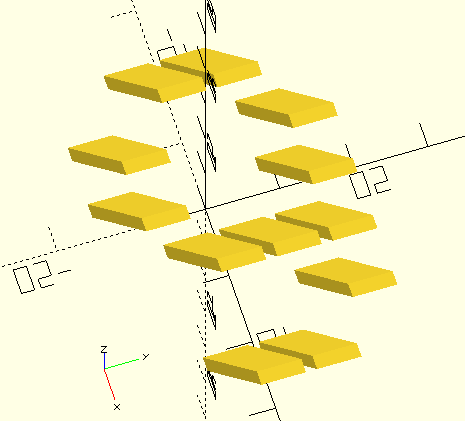
\includegraphics[height=.27\textwidth]{imagenes/nueve-60}}\hfill
  \subbottom[\lstinline!digito(120,8);!]
  {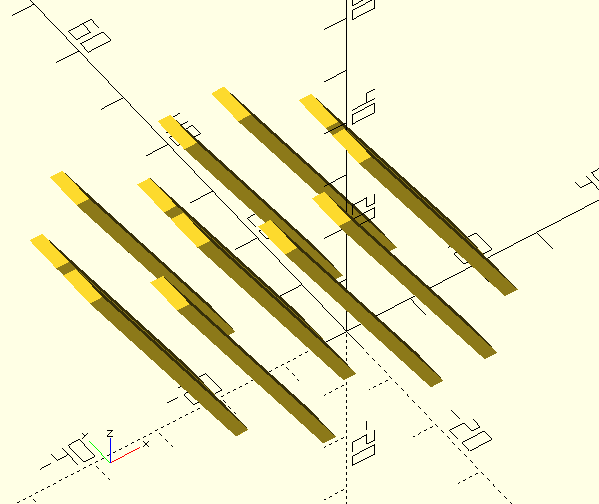
\includegraphics[height=.27\textwidth]{imagenes/ocho-120}}\hfill
  \subbottom[\lstinline!digito(20,7);!]
  {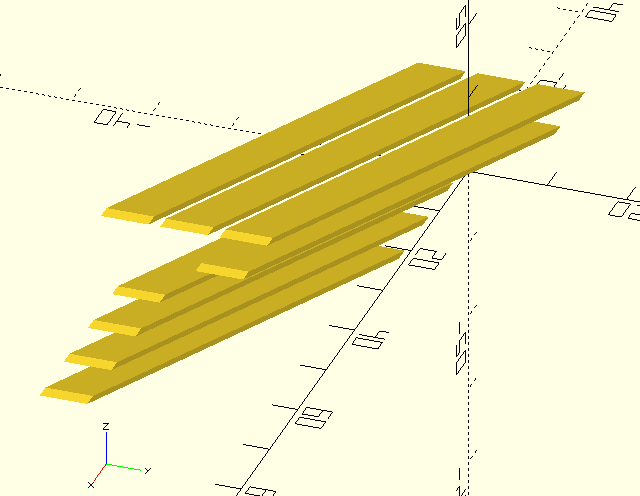
\includegraphics[height=.27\textwidth]{imagenes/siete-20}}
  \caption{Cecilia comprueba la corrección del módulo
    \lstinline!digito!.}%\iftoggle{libro}{}{\vspace{128in}}
  \label{fig:nueve-ocho-siete}
\end{figure}

La figura \ref{fig:nueve-ocho-siete} parecía asegurarle que sí.

  






%%% Local Variables:
%%% mode: latex
%%% TeX-master: "../libro"
%%% End:
